\section{RNNs and Language}

% Slide 21 - Meet Yoshua Bengio
\begin{frame}{Meet Yoshua Bengio}
    \begin{columns}
        \column{0.4\textwidth}
        % TODO: Add photo
        % 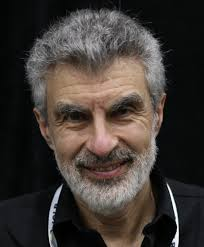
\includegraphics[width=\textwidth]{figures/bengio}
        
        \column{0.6\textwidth}
        \begin{itemize}
            \item \textbf{Most cited computer scientist globally}
            \item Most cited living scientist across all fields
            \item Neural probabilistic language model - \textbf{word embeddings}
        \end{itemize}
    \end{columns}
    
    \vspace{1em}
    \textit{``Third author. You know what's coming.''}
\end{frame}

% Slide 22 - The Language Problem
\begin{frame}{The Language Problem}
    \textbf{Old approach:} N-grams - counting symbol frequencies
    
    \vspace{1em}
    Number of possible N-grams: $V^N$ where $V$ = vocabulary size
    
    \vspace{1em}
    \begin{itemize}
        \item Brittle
        \item Slow
        \item No understanding of meaning
    \end{itemize}
\end{frame}

% Slide 23 - The Exponential Advantages
\begin{frame}{The Exponential Advantages of Deep Networks}
    Two reasons deep networks are powerful for language:
    
    \vspace{1em}
    \begin{enumerate}
        \item $n$ binary features $\rightarrow$ $2^n$ possible combinations
        
        \textit{``30 neurons can represent over a billion concepts''}
        
        \item Each layer \textbf{multiplies} expressive power exponentially
    \end{enumerate}
\end{frame}

% Slide 24 - Word Embeddings
\begin{frame}{Word Embeddings}
    \begin{itemize}
        \item \textbf{One-hot encoding:} one component = 1, rest = 0
        \item First layer creates activation patterns per word
        \item Foreshadows Word2Vec and modern embeddings
    \end{itemize}
    
    \vspace{1em}
    \textbf{Example:}
    \begin{itemize}
        \item Tuesday and Wednesday $\rightarrow$ similar vectors
        \item Sweden and Norway $\rightarrow$ similar vectors
    \end{itemize}
    
    \vspace{1em}
    \textit{``They didn't program it to learn this. It just did.''}
\end{frame}

% Slide 25 - Simple Feed Forward Language Model
\begin{frame}{Simple Feed Forward Language Model}
    \begin{itemize}
        \item Given 5 words, predict the next
        \item Works surprisingly well on:
        \begin{itemize}
            \item Small, clean datasets
            \item Large, messy real-world corpora
        \end{itemize}
    \end{itemize}
    
    \vspace{1em}
    \textbf{This was contrary to what people expected.}
\end{frame}

% Slide 26 - RNNs
\begin{frame}{Recurrent Neural Networks (RNNs)}
    \textbf{The problem:} Feed-forward networks can't handle sequences
    
    \vspace{1em}
    % TODO: Add RNN diagram (unrolled)
    
    \begin{itemize}
        \item Can translate English to French
        \item Learns semantic rules of both languages
        \item \textbf{Problem:} Vanishing gradient
    \end{itemize}
\end{frame}

% Slide 27 - LSTMs
\begin{frame}{Long Short-Term Memory (LSTM)}
    \textbf{Invented 1997}
    
    \vspace{1em}
    % TODO: Add LSTM cell diagram
    
    \begin{itemize}
        \item Cell state - long-term memory
        \item Gates - control information flow
        \item \textbf{Intuition:} Memory with a forget switch
    \end{itemize}
    
    \vspace{1em}
    The authors are bullish - and they're right.
\end{frame}

% Slide 28 - The Memory Bottleneck
\begin{frame}{The Memory Bottleneck}
    The biggest remaining problem:
    
    \vspace{1em}
    \begin{itemize}
        \item Neural networks are \textbf{stateless}
        \item Memory is inherently \textbf{stateful}
    \end{itemize}
    
    \vspace{1em}
    \textbf{Neural Turing Machines} (DeepMind, 2014)
    \begin{itemize}
        \item Differentiable Turing machine
        \item Attention-based read/write to memory
    \end{itemize}
    
    \vspace{1em}
    \textit{``They've identified the exact problem. The solution is two years away.''}
\end{frame}
